\documentclass[a4paper,10.5pt,dvipdfmx]{jarticle}  %jsarticleでも良いかも
%--脚注の設定
\usepackage{natbib}
\bibpunct[, ]{(}{)}{;}{and}{}{,} %本文での引用の体裁はここで整えられるみたい
\bibliographystyle{apsr2006-2}   %このagsmは編集済みなので注意。ジャーナルが太字にならないようにしてる。ブログ参照。
\usepackage{amsmath}
%--余白の設定   http://pcwide-jp.blogspot.co.uk/2009/07/latex.html  より
\setlength{\topmargin}{20mm}
\addtolength{\topmargin}{-1in}
\setlength{\oddsidemargin}{20mm}
\addtolength{\oddsidemargin}{-1in}
\setlength{\evensidemargin}{15mm}
\addtolength{\evensidemargin}{-1in}
\setlength{\textwidth}{170mm}
\setlength{\textheight}{254mm}
\setlength{\headsep}{0mm}
\setlength{\headheight}{0mm}
\setlength{\topskip}{0mm}
%--図の設定
%\usepackage[dvipdfmx]{graphicx} % PDFの利用もOKに
%\graphicspath{{./figures/}} %To add paths relative to the latexfile invoking the command
  %\usepackage[dvips]{graphicx}
%--行間の設定
\usepackage{setspace} 
\setstretch{1.13} % ページ全体の行間を設定
%コードの設定
\usepackage{listings}
\usepackage{color}
\definecolor{dkgreen}{rgb}{0,0.6,0}
\definecolor{mygray}{rgb}{0.5,0.5,0.5}
\definecolor{mauve}{rgb}{0.58,0,0.82}

\definecolor{codegreen}{rgb}{0,0.6,0}
\definecolor{codegray}{rgb}{0.5,0.5,0.5}
\definecolor{codepurple}{rgb}{0.58,0,0.82}
\definecolor{backgroundcolour}{rgb}{0.95,0.95,0.92}

\lstdefinestyle{Python} {
  language= Python, %ここを含めなければ、変に太字になったりしない
  aboveskip=2.5mm,
  belowskip=4.5mm,
  showstringspaces=false,
  columns=flexible,
  keepspaces=true,
  numbers=left,                    
  numbersep=5pt,    
  basicstyle={\small\ttfamily},
  commentstyle={\small\ttfamily},
  breaklines=true,
  breakatwhitespace=true
  tabsize=3
  backgroundcolor=\color{backgroundcolour},   
  commentstyle=\color{codegreen},
  keywordstyle=\color{magenta},
  numberstyle=\tiny\color{codegray},
  stringstyle=\color{codepurple},
	xleftmargin = 1.1cm,
  framexleftmargin = 1em
}
\lstdefinestyle{C} {
  language= C, %ここを含めなければ、変に太字になったりしない
  aboveskip=2.5mm,
  belowskip=4.5mm,
  showstringspaces=false,
  columns=flexible,
  keepspaces=true,
  numbers=left,                    
  numbersep=5pt,    
  basicstyle={\small\ttfamily},
  commentstyle={\small\ttfamily},
  breaklines=true,
  breakatwhitespace=true
  tabsize=3
  backgroundcolor=\color{backgroundcolour},   
  commentstyle=\color{codegreen},
  keywordstyle=\color{magenta},
  numberstyle=\tiny\color{codegray},
  stringstyle=\color{codepurple},
	xleftmargin = 1.1cm,
  framexleftmargin = 1em
}
\usepackage{xcolor}
\usepackage{framed}
\colorlet{shadecolor}{green!8}
%リンクの埋め込みを可能にする  \href{ **URL** }{表示テキスト}
\usepackage[dvipdfmx]{hyperref}
\usepackage{courier}
\usepackage{here}
%日本語環境用の設定を追加
\usepackage[english]{babel}
\renewcommand{\refname}{参考文献}
\renewcommand{\abstractname}{要約}
\usepackage{multirow}
\usepackage{placeins}
%数学用のフォント
\usepackage{amsmath} 
\usepackage{amssymb}
\usepackage{amsfonts} 
%tikz
\usepackage{tikz}
\usetikzlibrary{bayesnet}
%tightlist
\def\tightlist{
	\itemsep1pt
	\parskip1pt
	\parsep1pt
	\itemindent20pt
}
%subsubsubsection
\makeatletter
  \newcommand{\subsubsubsection}{\@startsection{paragraph}{4}{\z@}%
    {1.0\Cvs \@plus.5\Cdp \@minus.2\Cdp}%
    {.1\Cvs \@plus.3\Cdp}%
    {\reset@font\normalsize}
  }
  \makeatother
  \setcounter{secnumdepth}{4}
%statistically independent
\newcommand{\indep}{\mathop{\perp\!\!\!\!\perp}}
%-----------------
\begin{document}

\title{Variational Bayes Derivation of Poisson Mixture Model}
\author{@Shusei-E}
\maketitle
%\begin{abstract}
%\end{abstract}

\section{Model}
\begin{figure}[H]
\centering
\begin{tikzpicture}

  % Nodes

  \node[obs]                   (x)      {$x$} ; %
  \node[latent, left=of x]    (z)      {$z$} ; %
  \node[latent, left=of z]    (pi)  {$\pi$}; %
  \node[latent, left=of pi] (alpha) {$\alpha$};
  \node[latent, below=of z] (lambda) {$\lambda$};
	\node[latent, left=of lambda] (a) {$a$};
	\node[latent, below=of lambda] (b) {$b$};

	% Edges
	\edge{alpha}{pi}; \edge{pi}{z}; \edge{lambda}{x}; \edge{z}{x}; 
\edge{a}{lambda}; \edge{b}{lambda};

	% Plates
  \plate {plateN} { %
    (z)(x) %
  }{$N$}; %
	\plate{plateK}{
		(lambda)
	}{$K$};
\end{tikzpicture}
\caption{Poisson Mixture Model}
\end{figure}
\noindent
Variables:
\begin{itemize}
	\tightlist
	\item $N$: the number of data
	\item $D$: dimension
	\item $K$: the number of cluster
	\item $x$: data, $D \times N$ matrix
	\item $z$: latent category, $K \times N$ matrix
	\item $\lambda$: average parameter of Poisson distribution, $K \times D$ (each cluster has $D$ parameters)
	\item $\pi$: mixture coefficient, $K$ dimension
\end{itemize}
Data Generating Process:
\begin{align}
	p(\pi) &= {\rm Dir}(\pi | \alpha)\\
	p(\lambda) &= \prod_{k=1}^{K} \prod_{d=1}^{D} {\rm Gam} (\lambda_{d}^{(k)} | a,b)\\
	p(z|\pi) &= \prod_{n=1}^{N} {\rm Cat}(z_n | \pi)\\
	p(x | z, \lambda) &= \prod_{n=1}^{N} \prod_{k=1}^{K} \prod_{d=1}^{D} {\rm Poi} (x_{n,d} | \lambda_{d}^{(k)})^{z_{n}^{(k)}} \label{DGP:Poisson}
\end{align}
K-of-1 encoding is used for $z_n$. In Equation (\ref{DGP:Poisson}), $z_n$ takes $1$ for a certain $k$, so $z_n$ is a "switch" for Poisson distribution.

\section{Derivation}
\subsection{Induced Factorization}
Assuming $q(A,B,C) = q(A,B) q(C)$, $q(A,B) = q(A)q(B)$ is true if $A \indep B | X, C$. In this case, we can say $\lambda \indep \pi | x, c$ from the graphical model, so assuming $p(z, \lambda, \pi | x) \approx q(z) q(\lambda, \pi)$, induced factorization leads to $q(z) q(\lambda) q(\pi)$.

\subsection{Joint Distribution}
\begin{align}
	p(x, \pi, z, \lambda| \alpha, a, b) &= p(x| \pi, z, \lambda, \alpha ,a, b) p(\pi, z, \lambda | \alpha, a,b)\\
&= p(x| \pi, z, \lambda, \alpha ,a, b) p(z| \pi, \lambda, \alpha, a, b) p(\lambda, \pi | \alpha, a, b)\\
&= p(x | z, \lambda) p(z | \pi) p(\lambda | a, b) p(\pi | \alpha) \qquad {\rm (\because graphical\ model)}\\
&= \left[ \prod_{n=1}^{N} p(x_i | \lambda_{z_i=k}) p(z_i = k | \pi)  \right] \left[ \prod_{k=1}^{K} p(\lambda_k| a,b)  \right]   p(\pi | \alpha) 
\end{align}

\subsection{Evidence lower bound}
\noindent
Keep in mind that from factorization assumption (and induced factorization):
\begin{equation}
	p(z, \lambda, \pi | x) \approx q(z) q(\lambda) q(\pi)
\end{equation}
\noindent
Evidence lower bound (ELBO) is:
\begin{align}
	F[q(\pi, z, \lambda)] &= \iint \sum_{z} q(z) q(\lambda) q(\pi) \log \frac{p(x|z,\lambda) p(z|\pi) p(\lambda|a,b) p(\pi | \alpha)}{q(z)q(\lambda)q(\pi)} d\pi d\lambda\\
\begin{split}
&= \iint \sum_{z} q(z) q(\lambda) q(\pi) \log \left\{p(x|z, \lambda) p(z|\pi) \right\} d\pi d\lambda \\ &\quad - \sum_{z} q(z) \log q(z) + \int q(\pi) \log \frac{p(\pi | \alpha)}{q(\pi)} d\pi + \int q(\lambda) \log \frac{p(\lambda|a,b)}{q(\lambda)} d\lambda
\end{split}\\
\begin{split}
	&= \iint \sum_{i=1}^{N} \sum_{k=1}^{K} q(z_i = k) q(\lambda_k) q(\pi) \log \left\{p(x_{i}^{(k)}|\lambda_{z_i=k}) p(z_i = k|\pi) \right\} d\pi d\lambda \\ &\quad - \sum_{i=1}^{K} \sum_{k=1}^{K} q(z_i = k) \log q(z_i=k) + \underbrace{  \int q(\pi) \log \frac{p(\pi | \alpha)}{q(\pi)} d\pi  }_{{\rm KL}[q(\pi) || p(\pi|\alpha)]} + \sum_{k=1}^{K} \underbrace{ \int q(\lambda_k) \log \frac{ p(\lambda_k | a, b)}{ q(\lambda_k) } d \lambda_k  }_{ {\rm KL}[q(\lambda_k) || p(\lambda_k | a, b)]    } 
\end{split}
\end{align}


\section{Update Equation of $q(\pi)$}
%\subsection{Derivation}
\begin{align}
	\widetilde{F}[q(\pi)] = \int \sum_{i=1}^{N} q(\pi) \log \left\{ p(z_i=k | \pi) \right\} d\pi + \int q(\pi) \log \frac{p(\pi|\alpha)}{q(\pi)} d\pi
\end{align}
Using variational inference,
\begin{align}
	\frac{\delta \widetilde{F}[q(\pi)]}{\delta q(\pi)} = \frac{\partial \widetilde{F}[q(\pi)]}{\partial q(\pi)} &= \sum_{i=1}^{N} \log p(z_i = k | \pi) + \log \frac{p(\pi | \alpha)}{q(\pi)} - 1 = 0\\
	\Longleftrightarrow \qquad  \qquad  \qquad \log q(\pi) &\propto \sum_{i=1}^{N} \log p(z_i=k | \pi) + \log p(\pi | \alpha) \\
&= \log \left[ \left\{ \prod_{i=1}^{N} p(z_i=k | \pi)   \right\} p(\pi | \alpha) \right]\\
\Longleftrightarrow \qquad \quad \qquad  \qquad  q(\pi) &\propto \exp \left[ \log \left\{ \prod_{k=1}^{K} \pi_{k}^{\alpha_k -1} \prod_{i=1}^{N} p(z_i = k | \pi)  \right\} \right] \\
&= \exp \left[ \log \left\{ \prod_{k=1}^{K} \pi_{k}^{\alpha_k -1} \prod_{i=1}^{N} \pi_{k}^{z_i=k}  \right\} \right]\\
&= \exp \left[ \sum_{i=1}^{N} \sum_{k=1}^{K} \log (\pi_k)^{(\alpha_k -1)(z_i = k)}  \right]\\
&= \prod_{k=1}^{K} \pi_{k}^{\alpha_k - 1 + \sum_{i=1}^{N} (z_i=k)} \\
&= {\rm Dir} (\pi | \hat{\alpha}), \qquad \hat{\alpha} = \alpha_k + \sum_{i=1}^{N} (z_i=k)
\end{align}

Note:
\begin{align}
	\sum_{i=1}^3 \log a^{l_i} + \log_a^n &= \log a^{l_1} + \log a^{l_2} + \log a^{l_3} + \log a^n\\
&= \log a^{l_1 + l_2 + l_3 + n} \\
&= \log a^{\sum_{i=1}^3 l_i + n}
\end{align}

\section{Update Equation of $q(\lambda)$}
%\subsection{Derivation}
\noindent
\begin{align}
	\widetilde{F}[q (\lambda_k)] = \int \sum_{i=1}^{N} q(\lambda_k) \log \left\{ p(x_{i}^{(k)} | \lambda_{z_i=k}) \right\} d\lambda_k + \int q(\lambda_k) \log \frac{p(\lambda_k | a,b)}{q(\lambda_k)} d\lambda_k
\end{align}
\noindent
Recall distributions:
\begin{align}
	{\rm Gam}(\lambda_{d}^{(k)}|a,b) &= \frac{b^a}{\Gamma(a)} (\lambda_{d}^{(k)})^{a-1} \exp (-b \lambda_{d}^{(k)})\\
	{\rm Poi}(x, \lambda) &= \frac{e^{-\lambda} \lambda^x}{x!}
\end{align}
\noindent
Using variational inference,
\begin{align}
	\frac{\delta \widetilde{F}[q(\lambda_k)]}{\delta q(\lambda_k)} = \frac{\partial \widetilde{F}[q(\lambda_k)]}{\partial q(\lambda_k)} &= \sum_{i=1}^{N} \log p(x_{i}^{(k)} | \lambda_{z_i=k}) + \log \frac{p(\lambda_k|a,b)}{q(\lambda_k)} - 1 = 0\\
	\Longleftrightarrow \qquad  \qquad  \qquad \log q(\lambda_k) &\propto \sum_{i=1}^{N} \log p(x_{i}^{(k)} | \lambda_{z_i=k}) + \log p(\lambda_k | a,b)\\
	\Longleftrightarrow \quad  \qquad  \qquad \qquad q(\lambda_k) &\propto (\lambda_k)^{a-1} \exp (-b \lambda_k) \exp \left[ \sum_{i=1}^{N} \log p(x_{i}^{(k)} | \lambda_{z_i=k}) \right]\\
&= \exp \left[ \log \lambda_{k}^{a-1} \right] \exp (-b \lambda_k) \exp \left[ \sum_{i=1}^{N} \log e^{-\lambda_k} \lambda_k^{x_{i}^{(k)}} \right]\\
&= \exp \left[\log \lambda_{k}^{a-1}  - b \lambda_k + \sum_{i=1}^{N} \log \lambda_{k}^{x_{i}^{(k)}} + \sum_{i=1}^{N} \log e^{-\lambda_{z_i=k}} \right]\\
&= \exp \left[ \log \lambda_{k}^{a + \sum_{i=1}^{n} x_{i}^{(k)} -1 } + \left\{ - \left( b + \sum_{i=1}^{N} (z_i=k) \right) \lambda_k \right\} \right]
\end{align}
Recall $x_i^{(k)}$ infers we need to consider a "switch" for category, that is $z$.

\section{Update Equation of $q(z)$}
%\subsection{Derivation}
\noindent
\begin{align}
	\widetilde{F}[q (z)] = \sum_{i=1}^{N} q(z_i=k) \log \left\{ p(x_{i}^{(k)}) p(z_i=k|\pi) \right\} - \sum_{i=1}^{N} q(z_i=k) \log q(z_i=k)
\end{align}
\noindent
Using variational inference,
\begin{align}
	\frac{\delta \widetilde{F}[q(z)]}{\delta q(z)} = \frac{\partial \widetilde{F}[q(z)]}{\partial q(z)} &= \log \left\{ p(x_{i}^{(k)}) p(z_i=k|\pi) \right\} - \log q(z_i=k) - 1 = 0\\
	\Longleftrightarrow \qquad  \qquad  \qquad \log q(z_i=k) &\propto p(x_{i}^{(k)} | \lambda_{z_i=k}) p(z_i=k | \pi)\\
&= \left( e^{-\lambda_k} \lambda_{z_i=k}^{x_{i}^{(k)}} \right) \left( \prod_{k=1}^{K} \pi_{k}^{z_i=k} \right)\\
&= \prod_{d=1}^{D} \left( e^{-\lambda_{k,d}} \lambda_{z_i=k,d}^{x_{i,d}^{(k)}} \right) \left( \prod_{k=1}^{K} \pi_{k}^{z_i=k} \right)\\
&= \pi_k \exp \left[ \sum_{d=1}^{D} \left\{ - \lambda_{k,d} + x_{i,d}^{(k)} \log \lambda_{k, d}  \right\} \right]
\end{align}
Note that $\prod_{k=1}^{K} \pi_{k}^{z_i=k} = \pi_k$.

\section*{Reference}
\begin{enumerate}
	\item sammy-suyama「ベイズ混合モデルにおける近似推論1 ~変分近似~」 \url{http://machine-learning.hatenablog.com/entry/2016/07/06/200605}
\end{enumerate}

\end{document}
